\section{Objetivos}
\subsection{Objetivo General}

Explorar las interacciones entre genes y proteínas asociadas al Signo de Hoffman, utilizando bases de datos bioinformáticas y herramientas de análisis de redes para identificar posibles grupos funcionales y patrones de interacción relevantes.

\subsection{Objetivos Específicos}
\begin{enumerate}
	\item Identificar genes asociados al signo de Hoffman mediante la utilización de la Human Phenotype Ontology (HPO) y otras bases de datos relevantes.
	\item Construir una red de interacciones proteína-proteína (PPI) basada en los genes obtenidos, utilizando StringDB para analizar las interacciones de las proteínas codificadas por estos genes.
	\item Aplicar algoritmos de análisis de redes, como iGraph, para calcular métricas topológicas y determinar características clave de la red.
	\item Aplicar clustering en la red de interacción para identificar grupos de genes o proteínas que presenten una alta conectividad.
	\item Determinar las principales funciones biológicas y vías metabólicas en las que están involucrados los genes identificados mediante enriquecimiento funcional.
\end{enumerate}

\section{Materiales y Herramientas}

El estudio se apoyó en diversas herramientas, bases de datos especializadas y lenguajes de programación. Para aplicar preprocesamiento de datos biológicos y lograr un buen análisis de redes. A continuación, se detalla cada uno de los materiales empleados para la realización de este trabajo.

\subsection{Bases de datos}

\subsubsection{Human Phenotype Ontology (HPO)}
Es una base de datos que estandariza la representación de los fenotipos clínicos humanos y proporciona anotaciones de genes y enfermedades asociadas a cada fenotipo\cite{gargano2024}. Se utilizó HPO para identificar genes asociados al Signo de Hoffman, como parte del análisis de las interacciones genéticas. La ontología HPO fue fundamental para explorar las conexiones entre el Signo de Hoffman y diversos genes. Las consultas se realizaron mediante la API de HPO para obtener conjuntos de genes asociados a fenotipos de interés.

\subsubsection{StringDB}
La base de datos STRING (\textit{Search Tool for the Retrieval of Interacting Genes/Proteins}) se utilizó para construir redes de interacciones proteína-proteína (PPI) a partir de los genes identificados con HPO. STRINGDB es una base de datos que integra datos experimentales, predicciones computacionales y literatura científica para proporcionar información sobre interacciones proteicas \cite{szklarczyk2019}. A través de la API de StringDB, se obtuvo redes de interacción que sirvieron como base para los análisis de conectividad y agrupamiento de proteínas.

\subsection{Lenguajes de Programación}

\subsubsection{R}
El lenguaje de programación \textit{R} se utilizó en diferentes etapas del análisis, principalmente para el procesamiento de datos, la realización de análisis estadísticos y la visualización gráfica de resultados, específicamente fue usado la versión 4.3.3. R es ampliamente utilizado en bioinformática debido a su potente ecosistema de paquetes y librerías diseñados para el análisis de datos biológicos\cite{chan2018}. En este trabajo, R fue empleado para manipular los conjuntos de genes obtenidos. Las librerías utilizadas son:


\paragraph{Manipulación y Visualización de Datos:}
\begin{itemize}
	\item \textbf{tidyverse}: Conjunto de paquetes (incluyendo \textit{dplyr} y \textit{ggplot2}) que permiten manipular y graficar datos. \textit{dplyr} facilita el manejo de grandes datasets, mientras que \textit{ggplot2} permite generar gráficos de alta calidad \cite{Wickham2019}.
\end{itemize}

\paragraph{Análisis Bioinformático:}
\begin{itemize}
	\item \textbf{Bioconductor}: Conjunto de paquetes especializados en el análisis de datos genómicos. Fue utilizado para realizar análisis detallados de genes y anotaciones fenotípicas en el contexto del Signo de Hoffman \cite{Huber2015}.
	\item \textbf{iGraph para R}: Versión de iGraph en R, utilizada para la comparación de redes de interacción generadas en Python y el análisis estadístico de propiedades de red \cite{Csardi2006}.
\end{itemize}


\subsubsection{Python}
El lenguaje de programación \textit{Python} fue clave para la automatización de tareas, consultas a bases de datos, y análisis de redes. Python cuenta con un extenso conjunto de librerías que facilitan tanto la extracción de datos desde APIs como el análisis y modelado de redes. A continuación, se describen las librerías específicas empleadas en este estudio:

\paragraph{Análisis de Redes y Grafos:}
\begin{itemize}
	\item \textbf{iGraph}: Utilizada en el cálculo de métricas topológicas, análisis de comunidades y otras manipulaciones de redes complejas \cite{igraph2006}.
	\item \textbf{NetworkX}: Empleada como complemento de iGraph para la visualización y análisis interactivo de grafos, permitiendo inspeccionar la estructura y propiedades de redes de interacción proteína-proteína (PPI) \cite{hagberg2008}.
\end{itemize}

\paragraph{Visualización de Datos:}
\begin{itemize}
	\item \textbf{Matplotlib}: Proporciona las bases para crear gráficos y representaciones visuales básicas en Python, utilizadas en la representación gráfica de resultados bioinformáticos \cite{Hunter2007}.
	\item \textbf{Seaborn}: Ofrece una visualización de datos avanzada y estilizada, ideal para gráficos estadísticos que ayudan a visualizar las propiedades estructurales de redes y distribuciones de datos \cite{Waskom2021}.
\end{itemize}

\paragraph{Extracción y Manipulación de Datos:}
\begin{itemize}
	\item \textbf{Requests}: Se utilizó para realizar consultas a APIs como HPO y StringDB, a fin de recuperar datos de interacciones y anotaciones genéticas necesarias para los análisis \cite{Requests2020}.
	\item \textbf{Pandas}: Herramienta de manipulación de datos, utilizada para estructurar y limpiar datos previos a su análisis en redes. Facilita la gestión de grandes volúmenes de datos de genes y proteínas \cite{McKinney2010}.
\end{itemize}




\subsection{Software y Herramientas Computacionales}

\subsubsection{Entornos de Programación y Computación}
Para el desarrollo de los scripts y la ejecución de los análisis, se utilizó un entorno de programación basado en \textit{Jupyter Notebooks}, un entorno interactivo que facilita la escritura de código Python y la generación de gráficos en tiempo real. Los Notebooks son una herramienta ideal para integrar código, resultados y anotaciones de manera clara y ordenada.

Además, se emplearon editores de texto como \textit{Visual Studio Code} y \textit{RStudio} para escribir y depurar el código en Python y R, respectivamente. Ambos entornos ofrecen características avanzadas de edición.

\subsubsection{GitHub}
El control de versiones y la gestión de código se realizó mediante la plataforma \textit{GitHub}. A través de GitHub, se gestionaron los scripts de Python y R, así como los datos intermedios generados durante el análisis. GitHub es una plataforma de desarrollo colaborativo de software que permite a los usuarios almacenar, compartir y gestionar proyectos de código abierto. En el contexto de la bioinformática, GitHub se utiliza como una medida del impacto y la difusión de software, ya que proporciona estadísticas sobre el uso de repositorios, contribuciones de usuarios y la popularidad de diferentes proyectos\cite{dozmorov2018}. 


\subsubsection{API de HPO y StringDB}
La API de \textit{Human Phenotype Ontology (HPO)} y la API de \textit{StringDB} hace falta mencioanr las API por separado?

\subsection{Algoritmos de Análisis}

\textbf{!!!CAMBIAR CUANDO HAGAMOS METODOLOGIA}

Para evaluar las redes de interacción obtenidas y realizar el análisis de agrupamiento, se utilizaron diversos algoritmos implementados en las librerías antes mencionadas. Cada algoritmo contribuye de manera única al análisis de la estructura y conectividad de las redes de interacción, permitiendo detectar patrones y comunidades relevantes en el contexto de las redes proteína-proteína.
\\

\begin{itemize}
	\item \textbf{Algoritmo de Clustering (Louvain)}: Este algoritmo optimiza la partición de una red maximizando su modularidad, lo cual es especialmente útil en redes grandes y complejas. Es ampliamente utilizado para detectar comunidades en redes biológicas, proporcionando un análisis modular efectivo de interacciones genéticas \cite{Blondel2008}.
	
	\item \textbf{Algoritmo de Girvan-Newman}: Este algoritmo detecta comunidades en redes complejas mediante la eliminación iterativa de enlaces con la mayor intermediación, revelando así la estructura modular subyacente. Es particularmente útil en redes densas donde se busca identificar patrones de comunidades \cite{Girvan2002}.
	
	\item \textbf{Algoritmo de Optimización Voraz}: Este enfoque de resolución de problemas realiza decisiones locales en cada paso, eligiendo la opción más beneficiosa sin considerar impactos a largo plazo. Utilizado para maximizar la modularidad en redes, es eficaz para identificar comunidades cuando se requieren decisiones rápidas \cite{Fortunato2010}.
	
	\item \textbf{Propagación de Etiquetas}: Este algoritmo agrupa datos según su similitud, sin la necesidad de especificar el número de clústeres a priori, haciéndolo adecuado para una exploración inicial de la estructura de la red \cite{Raghavan2007}.
	
	\item \textbf{Métricas de Análisis de Redes}: Para caracterizar las propiedades estructurales de las redes generadas, se emplearon métricas como la centralidad de grado, el coeficiente de agrupamiento y la centralidad de intermediación. Estas métricas permiten comprender cómo los genes o proteínas se conectan entre sí dentro de la red y resaltar los nodos más relevantes en términos biológicos.
	
	\item \textbf{Enriquecimiento Funcional}: Una vez identificados los clusters, se realizó un análisis de enriquecimiento funcional para determinar qué funciones biológicas, rutas metabólicas o procesos celulares están sobrerrepresentados en los grupos de genes o proteínas detectados. 
\end{itemize}



\section{Métodos}

\subsection{Flujo de trabajo}

\begin{figure}[h!]
	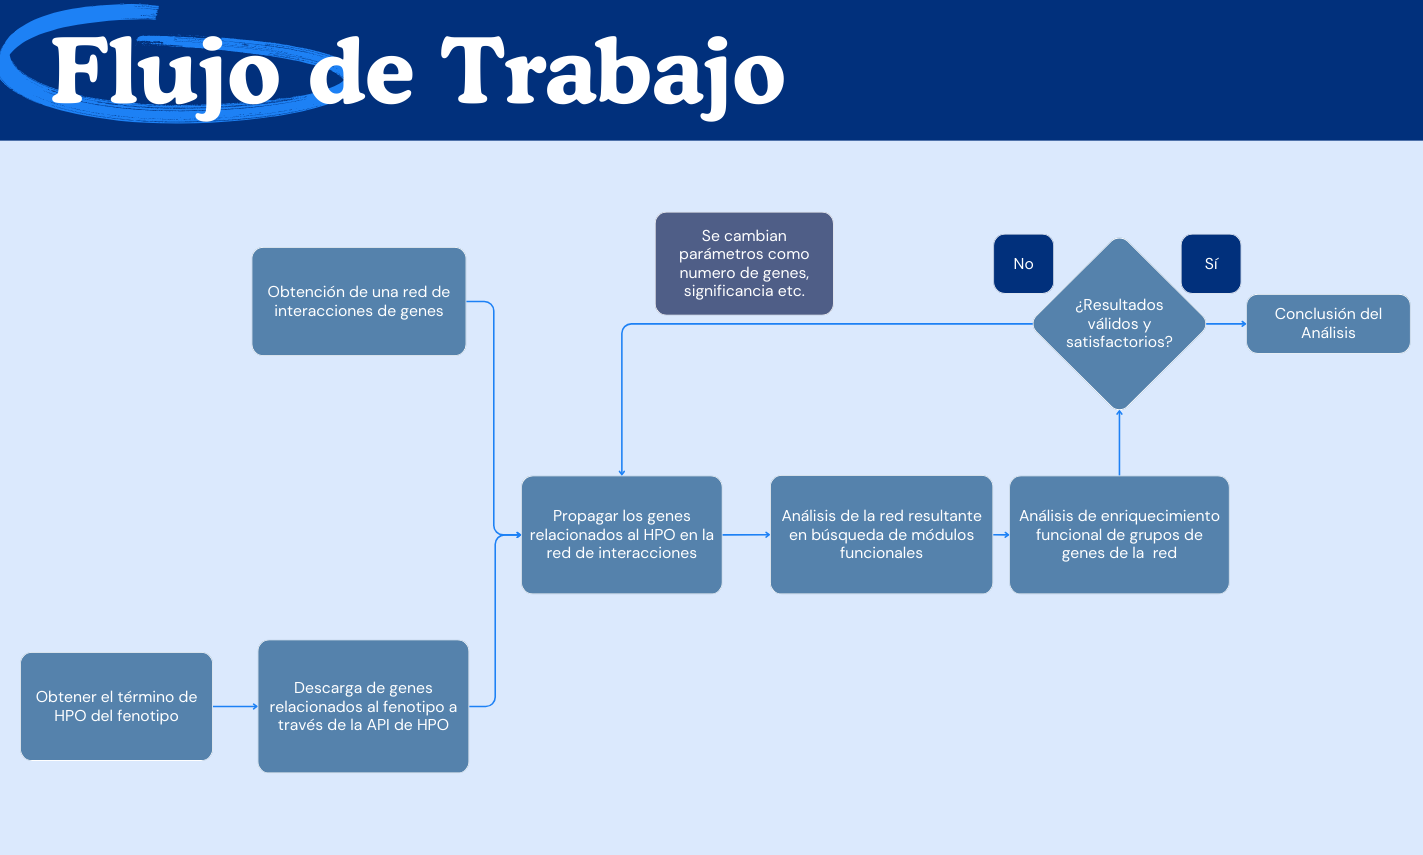
\includegraphics[width=.95\textwidth]{figures/workflow.png}
	\caption{Flujo de trabajo}
	\label{fig:workflow}
\end{figure}

\subsection{Obtención de genes relacionados con signo de Hoffman}

Se descargaron los genes relacionados con el termino HP:0031993 a través de la API de HPO a través del endpoint \url{https://ontology.jax.org/api/network/annotation/HP:0031993/download/gene} 
\subsection{Obtención de red de interacciones de genes}

Se descargó una red de interacciones génicas a partir de la base de datos STRING. Posteriormente, los identificadores de las proteínas se transformaron a identificadores estándar HUGO.

\subsection{Propagación de red}

Se utilizó el algoritmo DIAMoND para propagar los genes relacionados con el fenotipo de signo de hoffman en la red de interacciones con el objetivo de formar una subred de genes relacionadas con el signo de hoffman.

\subsection{Análisis de red}

Para identificar módulos funcionales en la red, aplicaremos el algoritmo de Louvain, que es un método eficiente para detectar comunidades en redes grandes. Este algoritmo agrupa nodos en función de la densidad de sus interacciones, dividiendo la red en clusters que representan módulos con una alta cohesión interna. Cada módulo contiene genes que están más conectados entre sí que con otros nodos de la red, lo que permite identificar posibles grupos funcionales.

Luego, calcularemos métricas topológicas para analizar la estructura y el rol de los genes en la red. Primero, la centralidad de grado nos indicará qué tan conectado está cada gen dentro de la red; este valor es útil para identificar nodos bien conectados dentro de sus módulos. La centralidad de intermediación nos permitirá ver cuáles genes son críticos en el flujo de información, actuando como puentes o enlaces entre distintos módulos. Por último, la centralidad de cercanía nos ayuda a ver qué tan rápidamente un gen puede acceder a otros genes en la red, indicando nodos que son importantes para la cohesión interna del módulo.

Este análisis topológico ayuda a identificar los genes más relevantes de cada módulo. Al final, tendremos una red dividida en módulos funcionales que representan grupos de genes potencialmente parecidos en términos biológicos.

\subsection{Análisis de enriquecimiento funcional}

Una vez identificados los clusters, se realizó un análisis de enriquecimiento funcional para determinar qué funciones biológicas, rutas metabólicas o procesos celulares están sobrerrepresentados en los grupos de genes detectados.